\documentclass{beamer}
\usepackage{amsmath}
\usepackage{euler}
\usepackage{graphicx}
\usepackage{subcaption}
\usepackage{hyperref}
\usepackage{amsfonts, amsmath, amssymb}
\usetheme[progressbar = frametitle]{metropolis}
\setbeamertemplate{frame numbering}[fraction]
\title{Development and testing of a python based Trajectory-Surface-Hopping code for simulating Non-adiabatic dynamics}
\author{Md. Elious Ali Mondal}
\date{}

\begin{document}
\metroset{block=fill}

	\begin{frame}
	\titlepage
	\end{frame}
	
	\begin{frame}[t]{The Born-Oppenheimer Approximation (BOA)}
	Due to heavy mass of the nuclei, we can quite accurately assume that the nuclear motion doesn't effect the electronic motion and thus we can seperate the electronic and nuclear degrees of freedom;
	\begin{equation}
	\hat{H}_{mol} = \hat{H}_{e^-} + \hat{H}_{Nu}
	\end{equation}
	due to which we can seperately solve for;
	\begin{equation}
	\hat{H}_{e^-}(\textbf{r};\textbf{R})\Psi_{e^-}(\textbf{r};\textbf{R}) = E_{e^-}(\textbf{R})\Psi_{e^-}(\textbf{r};\textbf{R})
	\end{equation}
	Here $\textbf{r}\rightarrow$ $e^-$ coordinates and $\textbf{R}\rightarrow$ Nuclear coordinates and in the above \textbf{R} is just a parameter.\\ $\hat{H}_{mol}$ depends on time through \textbf{R}(t).\\ $E_{e^-}(\textbf{R})$ is called an electronic Potential Energy Surface (PES).
	\end{frame}	
	
	\begin{frame}[t]{Non-adiabatic processes, An example...}
	\begin{figure}
	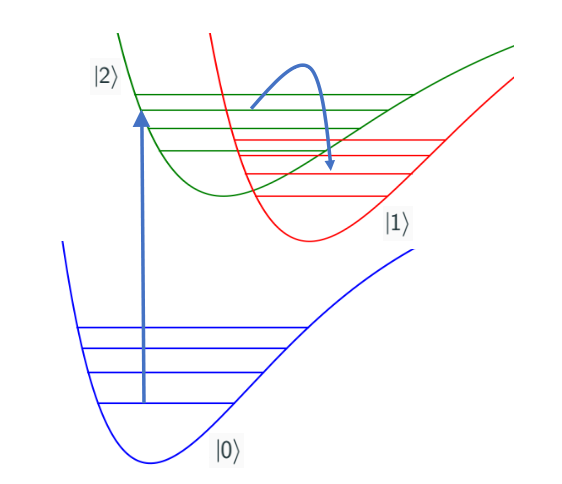
\includegraphics[scale=0.50]{NAD.png}
	\caption{Non-adiabaticity in excited states}
	\end{figure}
	\end{frame}
	
	\begin{frame}[t]{Origin of non-adiabaticity ....}
	Lets take our system to be in $i^{th}$ eigenstate, $\Psi_i$, of hamiltonian $\hat{H}$. The system evolves as;
	\begin{equation}
	i\hbar\frac{\partial \Psi_i}{\partial t} = \hat{H}\Psi_i
	\end{equation}
	Suppose at each instant of time, we have the instantaneous eigenbasis as;
	\begin{equation}
	\hat{H}(t)\phi_j(t) = E(t)\phi_j(t)
	\end{equation}
	Then we can represent out instantaneous wavefunction as;
	\begin{equation}
	\Psi_i(t) = \sum_i c_j(t)\phi_j(t)
	\end{equation}
    \end{frame}	
    
    \begin{frame}[t]{The non-adiabatic term...}
    We can show,
    \begin{equation}
    \underbrace{i\hbar\dot{c}_k(t) = c_k(t)E_k(t)}_\text{adiabatic part} - \underbrace{i\hbar \sum_jc_j\frac{\langle\phi_k|\dot{\hat{H}}|\phi_j\rangle}{E_j-E_k}}_\text{non-adiabatic part}
    \end{equation}
    So the non-adiabaticity can occur when:
    \begin{enumerate}
    \item{Instantaneous eigenvalues are nearly degenerate}
    \item{$|\dot{H}_{kj}| \geqslant |E_j-E_k|$}
    \end{enumerate}
    The non-adiabatic part of eqn(4) is also called the \textbf{Non-adiabatic coupling (NAC)} between different instantaneous eigenstates.
    \end{frame}  
    
    
	\begin{frame}[t]{Non-adiabatic coupling}
	\begin{figure}
	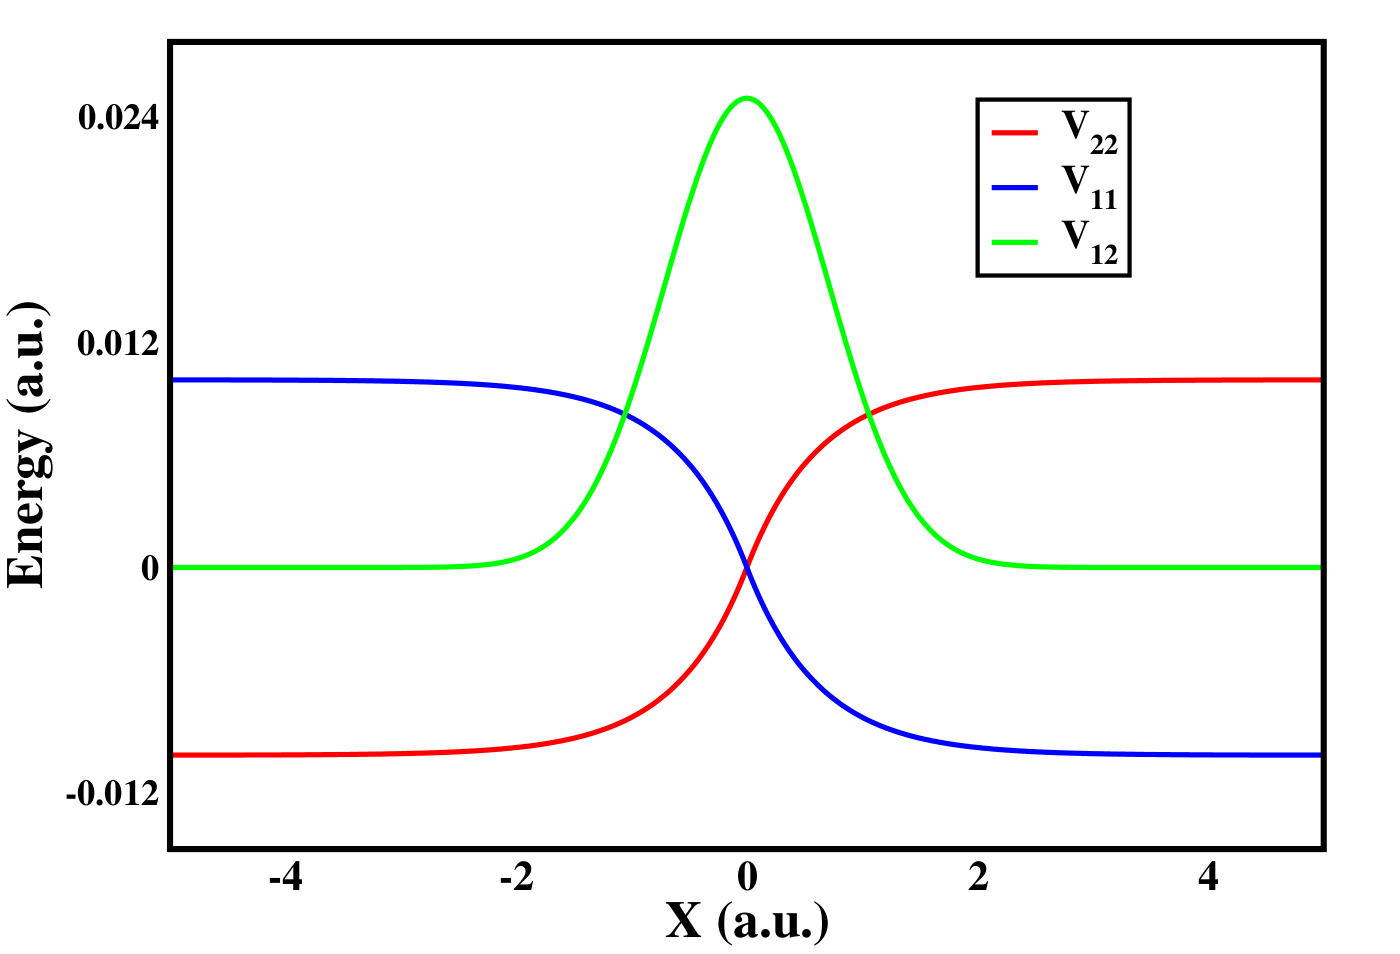
\includegraphics[scale=0.20]{NAC_elious.png}
	\caption{NAC}
	\end{figure}
	\end{frame}     	
	
	\begin{frame}[t]{What we want to simulate...}
	\begin{center}
	\begin{figure}
	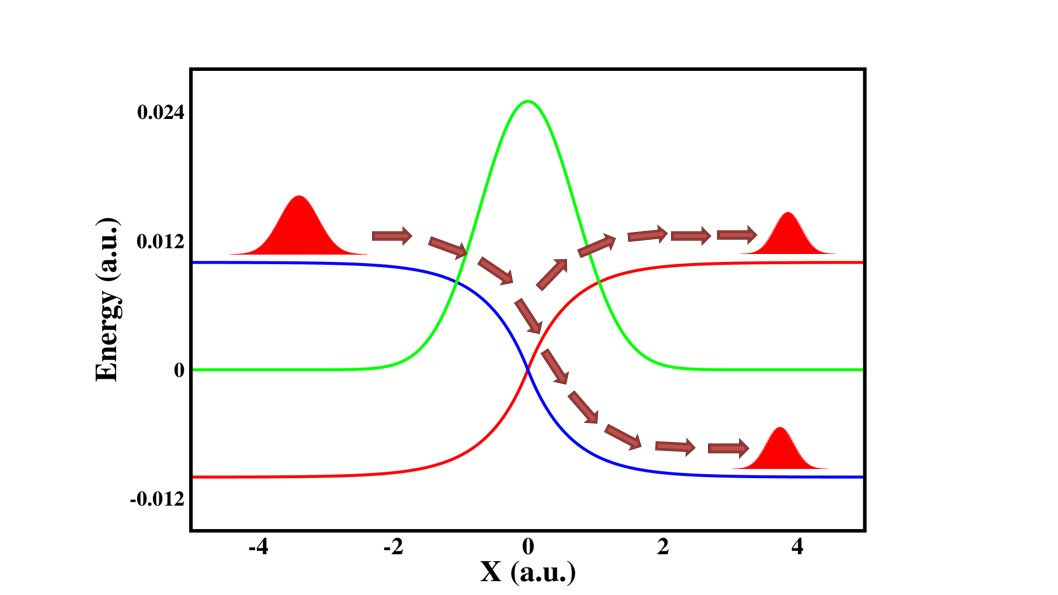
\includegraphics[width=1.1\linewidth, height=0.6\linewidth]{nuclear_propagation.jpg}
	\caption{Nuclear wavepacket propagation}
	\end{figure}
	\end{center}
	\end{frame}
	

	\begin{frame}[t]{Tully's Fewest-Switches-Surface-Hopping (FSSH)}
	\begin{enumerate}
	\item[1.]{We simulate an ensemble of independent-trajectories (\textbf{R}(t)) with different initial conditions.}
	\item[2.]{For each trajectory we assume the electronic wavefunction to be of the form:
	\begin{equation}
	\Psi(\textbf{r};\textbf{R}(t)) = \sum_kc_k(t)\Phi_k(\textbf{r};\textbf{R}(t))
	\end{equation}}
	\item[3.]{The nuclear coordinates evolve according to:
	\begin{equation}
	M_I\ddot{\textbf{R}} = -\nabla E_k(\textbf{R}(t))
	\end{equation}}
	\item[4.]{The electronic coefficients evolve according to eqn(4) which in density matrix notation;
	\begin{equation}
	i\hbar\dot{\rho}_{kj} = \rho_{kj}(E_k(\textbf{R})-E_j(\textbf{R})) - i\hbar \sum_l\left\lbrace\rho_{lj}\textbf{d}_{kl}\textbf{.}\dot{\textbf{R}} + \rho_{kl}\textbf{d}_{lj}\textbf{.}\dot{\textbf{R}}\right\rbrace
	\end{equation}}
	\end{enumerate}
	\end{frame}
	
	\begin{frame}[t]{FSSH continued...}
	where,
	\begin{equation}
	\textbf{d}_{mn} = \frac{\langle\Phi_m|\nabla_R\hat{H}|\Phi_n\rangle}{E_n-E_m}
	\end{equation}
	This is called the Non-Adiabatic coupling vector (NACV) between the different PES.
	The diagonals terms of the density matrix above are the populations;
	\begin{equation}
	\dot{\rho}_{kk} = -\sum_{l \neq k}2\text{Re}(\rho_{kl}^*\textbf{d}_{kl}\textbf{.}\dot{\textbf{R}}) = \sum_{l\neq k}\gamma_{kl}
	\end{equation}
	\begin{enumerate}
	\item[5]{At regions of strong coupling, we allow the trajectory to hop from one PES to another based on a stochstic algorithm.The probability of a hop $j\rightarrow k$ in between time \textit{t} and $t+dt$ is calculated by,
	}
	\end{enumerate} 
	\end{frame}
	
	\begin{frame}[t]{}
	\begin{equation}
	\begin{split}
P_{j\rightarrow k}(t) &= \frac{\text{change in population of k due to j}}{\text{population of j}}\\
&= max\left[0,\frac{\gamma_{kj}dt}{\rho_{jj}}\right]
\end{split}
	\end{equation}
	\begin{enumerate}
	\item[6.]{The switch from an electronic state \textit{j} to \textit{k} will occur if,
\begin{equation}
\sum_{m=1}^{k-1}P_{j\rightarrow m} < \zeta <  \sum_{m=1}^{k}P_{j\rightarrow m}
\end{equation}
where $\zeta$ is a random rumber between 0 and 1.}
	\end{enumerate}
	\end{frame}
	
	\begin{frame}[t]{FSSH algorithm}
	\begin{enumerate}
	\item[\textbf{Step1}]{Generate different initial conditions either by wigner sampling or by Molecular Dynamics.}
	\item[\textbf{Step2}]{Propagate the nuclei starting from an inital PES following eqn(8).}
	\item[\textbf{Step3}]{Calculate the NACs in eqn(4)}
	\item[\textbf{Step4}]{Propagate the electronic coefficients by eqn(4)}
	\item[\textbf{Step5}]{Calculate the hopping probability and decide the hop according to eqn(12) and (13).}
	\item[\textbf{Step6}]{If the hop occurs, change the PES and readjust the momentum along the NACV direction (if available) or distribute momentum uniformly. If no hop occurs, continue along the same PES}
	\item[\textbf{Step7}]{Repeat from \textbf{Step2} until a stopping criterion is reached.}
	\end{enumerate}		
	\end{frame}
	
	\begin{frame}[t]{Internal consistency of FSSH}
	Suppose we simulated $N^T$ number of trajectories and at any time step of the FSSH simulation, if we have $N^\alpha$ in the electronic state $\alpha$, then we should have:
    \begin{equation}
	\frac{N^\alpha}{N^T} = \frac{1}{N^T}\sum_{j=1}^{N^T} \rho_{\alpha\alpha}^j
	\end{equation}
	Eqn(14) is called the internal consistency of FSSH.\\
	\vspace{1cm}
	Tully's FSSH algorithm is known to be internally inconsistent. Lets understand why?...
	
	\end{frame}
	
	\begin{frame}[t]{How does overcoherence arise???}
	Consider the Born-Huang ansatz for total wavefunction of the combined nuclei-electron system:
	\begin{equation}
	|\Psi\rangle = \sum_i f_i|\chi_i\rangle|\phi_i\rangle 
	\end{equation}
	The density matrix will be;
	\begin{equation}
	|\Psi\rangle\langle\Psi| = \sum_{i,j} f_if_j^*|\chi_i\rangle|\phi_i\rangle \langle\phi_j|\langle\chi_j|
	\end{equation}
	Now to bring out the electronic density matrix from this;
	\begin{equation}
	\sigma_{el} = \sum_{i,j} f_if_j^*\displaystyle\int|\textbf{R}\rangle\langle\textbf{R}||\Psi\rangle\langle\Psi| d\textbf{R}
	\end{equation}
	\end{frame}

	\begin{frame}[t]{Overcoherence...}
	This would give;
	\begin{equation}
	\begin{split}
	\sigma_{el} &= \sum_{i,j} f_if_j^* \displaystyle\int \langle\chi_j|\textbf{R}\rangle\langle\textbf{R}|\chi_i\rangle|\phi_i\rangle\langle\phi_j| d\textbf{R}\\
	&= \sum_{i,j} f_if_j^* \langle\chi_j|\chi_i\rangle|\phi_i\rangle\langle\phi_j|
	\end{split}
	\end{equation}
	The electronic wavefunction in TSH is;
	\begin{equation}
	|\Psi_{el}\rangle = \sum_i c_i|\phi_i\rangle
	\end{equation}
	From this we have the electronic density matrix as;
	\begin{equation}
	\sigma_{el} = \sum_{i,j} c_ic_j^*|\phi_i\rangle\langle\phi_j|
	\end{equation}
    \end{frame}	
    
    \begin{frame}[t]{Overcoherence continued...}
    Comparing equations (18) and (20) we can see that the coherence terms in TSH wave-function  represents the nuclear overlap of the total-wavefunction, i.e.,
    \begin{equation}
    f_if_j^*\langle\chi_j|\chi_i\rangle = c_ic_j^*
    \end{equation} 
    \begin{enumerate}
    \item{After branching off of the nuclear wavepackets from strong coupling regions, when these wavepackets are far enough in phase space, then the effective overlap should go to 0 i.e., $\langle\chi_j|\chi_i\rangle \rightarrow 0$.}
    \item{BUT, there is no term in equation(eqn(9)) which will make the coherence terms $\rightarrow 0$ after the hops.}
    \item{This leads to overcoherence.}
	\end{enumerate}        
    \end{frame}
    
    \begin{frame}[t]{Instantaneous Decoherence Correction (IDC)}
	\begin{enumerate}
	\item{\textbf{ID-S:} After each successful hop, the electronic wavefunction is reinitialised as a pure state in the current state}
	\item{\textbf{ID-A:} If a hop is accepted, the wavefunction is made to collapse at the current state and if a hop is forbidden, the wavefunction is collapsed back to the current running state.}
	\end{enumerate}
	If a hop $S_2 \rightarrow S_1$ is predicted:\\
	\hspace{2cm} if successful hop:\\
	\hspace{4cm} set $c_1 = 1$ and $c_2 = 0$\\
	\hspace{2cm} else:\\
	\hspace{4cm} set $c_2 = 1$ and $c_1 = 0$\\
	\end{frame}
	
	\begin{frame}[t]{Energy Based Decoherence Correction (EDC)}
	Instead of instantaneous collapse, here we allow for decay of the electronic wavefunction to a particular state.
	\begin{equation}\label{eq:16}
	c_\beta'(t) = c_\beta(t)e^{\frac{-\Delta t}{\tau_{\beta\alpha}(t)}}
    \end{equation}
    and the loss gets accumulated in the current state as:
    \begin{equation}\label{eq:17}
    c_\alpha'(t) = c_\alpha(t)\left[\frac{1-\sum_{\beta\neq\alpha}|c_\beta'(t)|^2}{|c_\alpha'(t)|^2}\right]^{\frac{1}{2}}
    \end{equation}    	 
    $\tau_{\beta\alpha}$ is known as the decoherence time and Granucci \textit{et al.} approximated this to be:
    \begin{equation}\label{eq:19}
    \tau_{\beta\alpha}(t) = \frac{\hbar}{|E_\beta(t)-E_\alpha(t)|}\left(C+\frac{E_0}{E_{kin}}\right)
    \end{equation}
	\end{frame}  
	
	\begin{frame}
	\huge{\textbf{Thank You}}
    \end{frame}	  	
	
\end{document}